\documentclass{csse4400}

\usepackage{languages}

\title{AWS Academy Introduction}
\author{Brae Webb}

\date{\week{1}}
\begin{document}

\maketitle

\section{Before Class}
Prior to attending class, \textbf{select an open-source website} that you would be interested in deploying.
In this guide, we will be deploying hextris \cite{hextris}, an online game similar to tetris.
You may also deploy hextris, although,
you can take the opportunity choose something which interests you.
Note that deploying other websites is likely to be more involved than the example in the guide.

Potential ideas are:
\begin{itemize}
    \item \textbf{Habitica:} \url{https://github.com/HabitRPG/habitica}
    \item \textbf{DailyNotes:} \url{https://github.com/m0ngr31/DailyNotes/}
    \item \textbf{kcal:} \url{https://github.com/kcal-app/kcal} 
\end{itemize}

\noindent Alternatively, browse through the impressive collection here:\\ \url{https://github.com/awesome-selfhosted/awesome-selfhosted}

\section{This Week}
This week our goal is to get acquainted with AWS Academy.
Throughout the course we will use AWS Academy to learn how to deploy and manage infrastructure with AWS.
Specifically, this week you need to:
\begin{itemize}
    \item Enrol in
    \begin{enumerate}
        \item AWS Academy Cloud Foundations [10906] course;
        \item AWS Academy Learner Lab - Foundation Services [10909] course; and
    \end{enumerate}
    \item Navigate the AWS Academy interface.
    \item Enter the AWS Console from an AWS Academy lab.
    \item Use the AWS Console to provision an EC2 instance with a simple web interface.
\end{itemize}

\section{AWS Academy}
AWS Academy is an educational platform to support teaching AWS services.
In this course, we will be using it in two ways:
\begin{enumerate}
    \item The Cloud Foundations course will be used as supplementary material to help cement your ability to use AWS.
          The use of Cloud Foundations is completely optional.
    \item The Learner Lab provides access to an environment which will be used in these practicals to learn AWS. 
\end{enumerate}

\section{Enrol in AWS Academy}

\begin{enumerate}
    \item
        Set up your AWS Academy account by responding to your email invitation and clicking \textbf{Get Started}.
        The email invitation will come from AWS Academy.
        Check your junk/spam folders.

        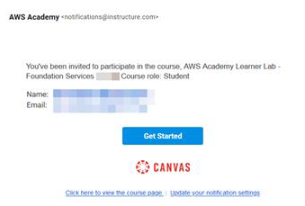
\includegraphics{images/email-invite}

    \item Go to \url{https://www.awsacademy.com/LMS_Login} to login.
    \begin{enumerate}
        \item Press \textbf{Student Login}.
        \item Use the email address that received the email invitation.
    \end{enumerate}

    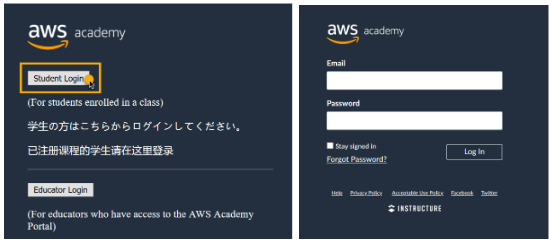
\includegraphics[width=0.75\textwidth]{images/labs-login}
\end{enumerate}


\section{Exploring the Interface}
\aside{We will just be looking at the learner lab today, please ask on the discussion board if you need help using the cloud foundations course.}

The following steps will enter the learner lab:

\begin{enumerate}

\item Once you have enrolled in the course, you should see this course page (minus everything in pink):

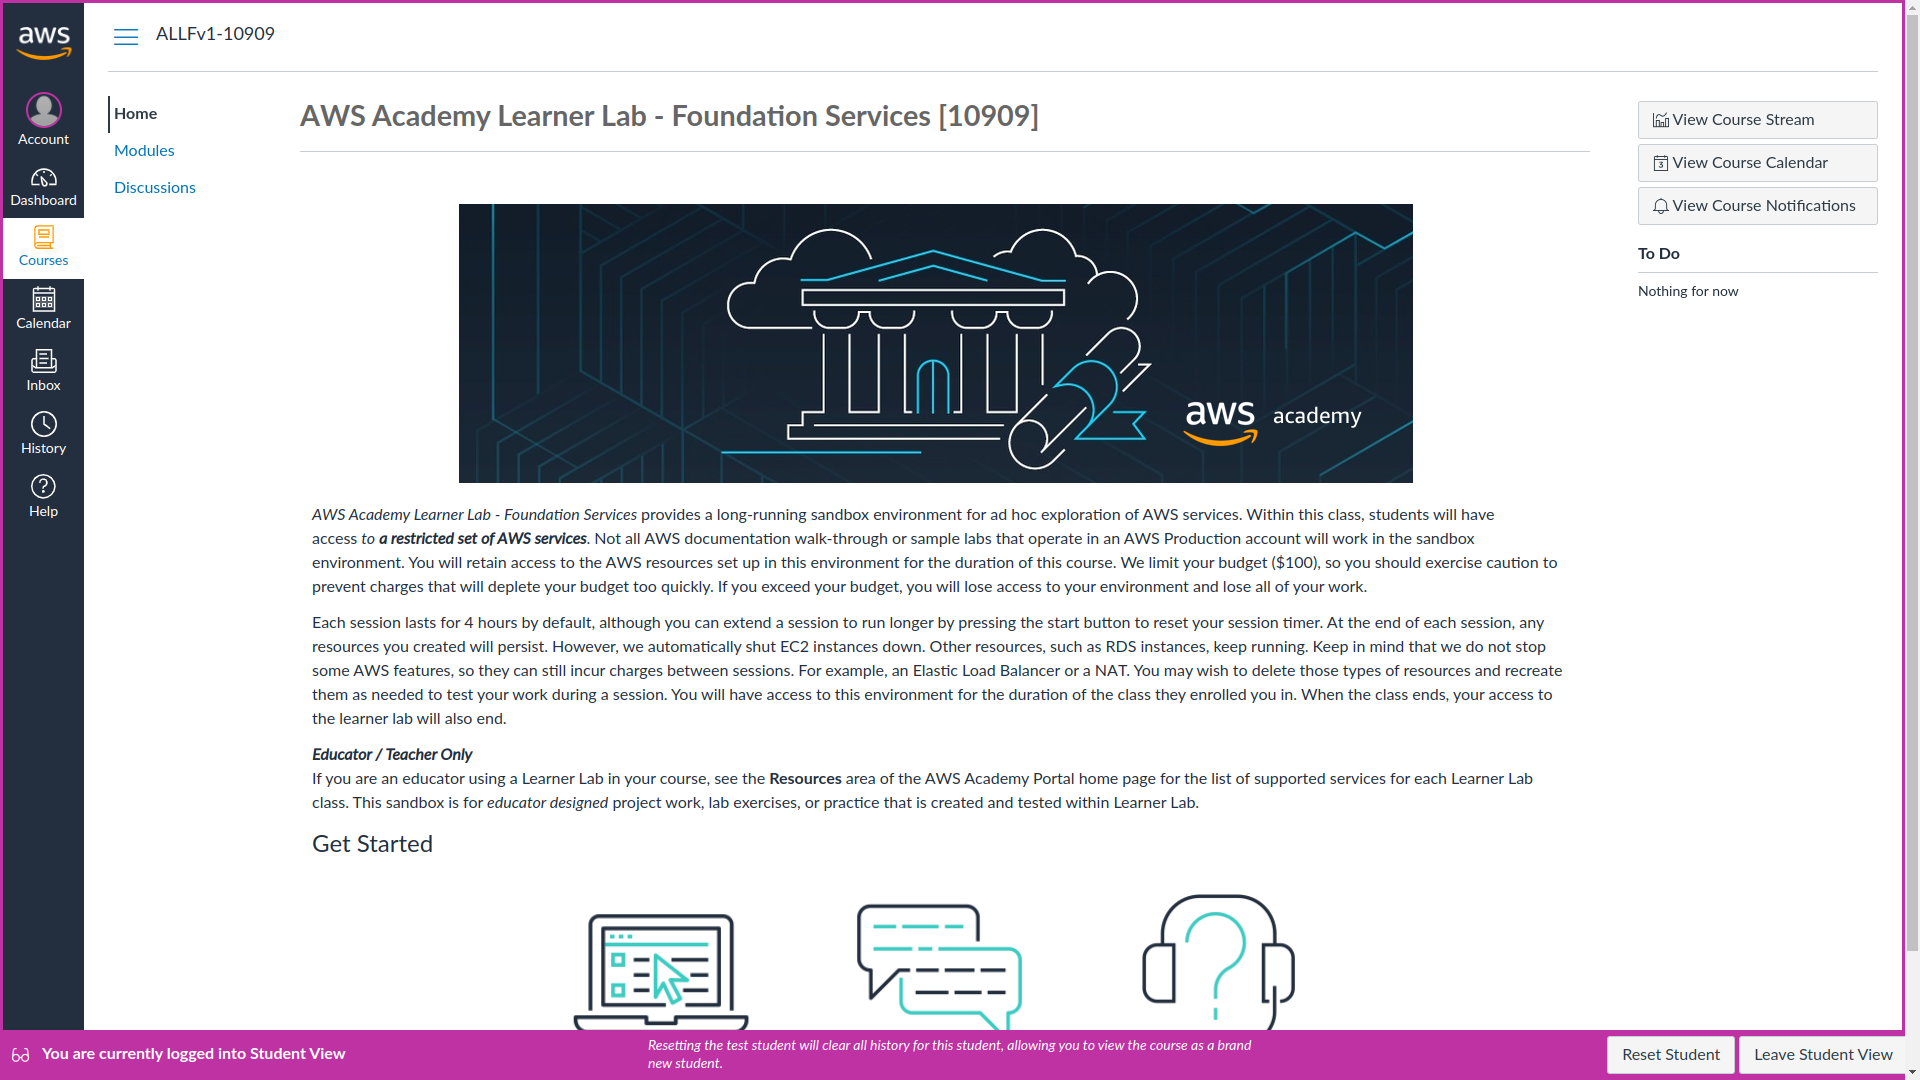
\includegraphics[width=0.9\textwidth]{images/academy-homepage}

\item Navigate to the \texttt{Modules} tab and select the link for ``Learner Lab - Foundational Services''.
      You may also open and browse the ``Learner Lab - Student Guide.pdf'' link which covers some of the content of this guide.

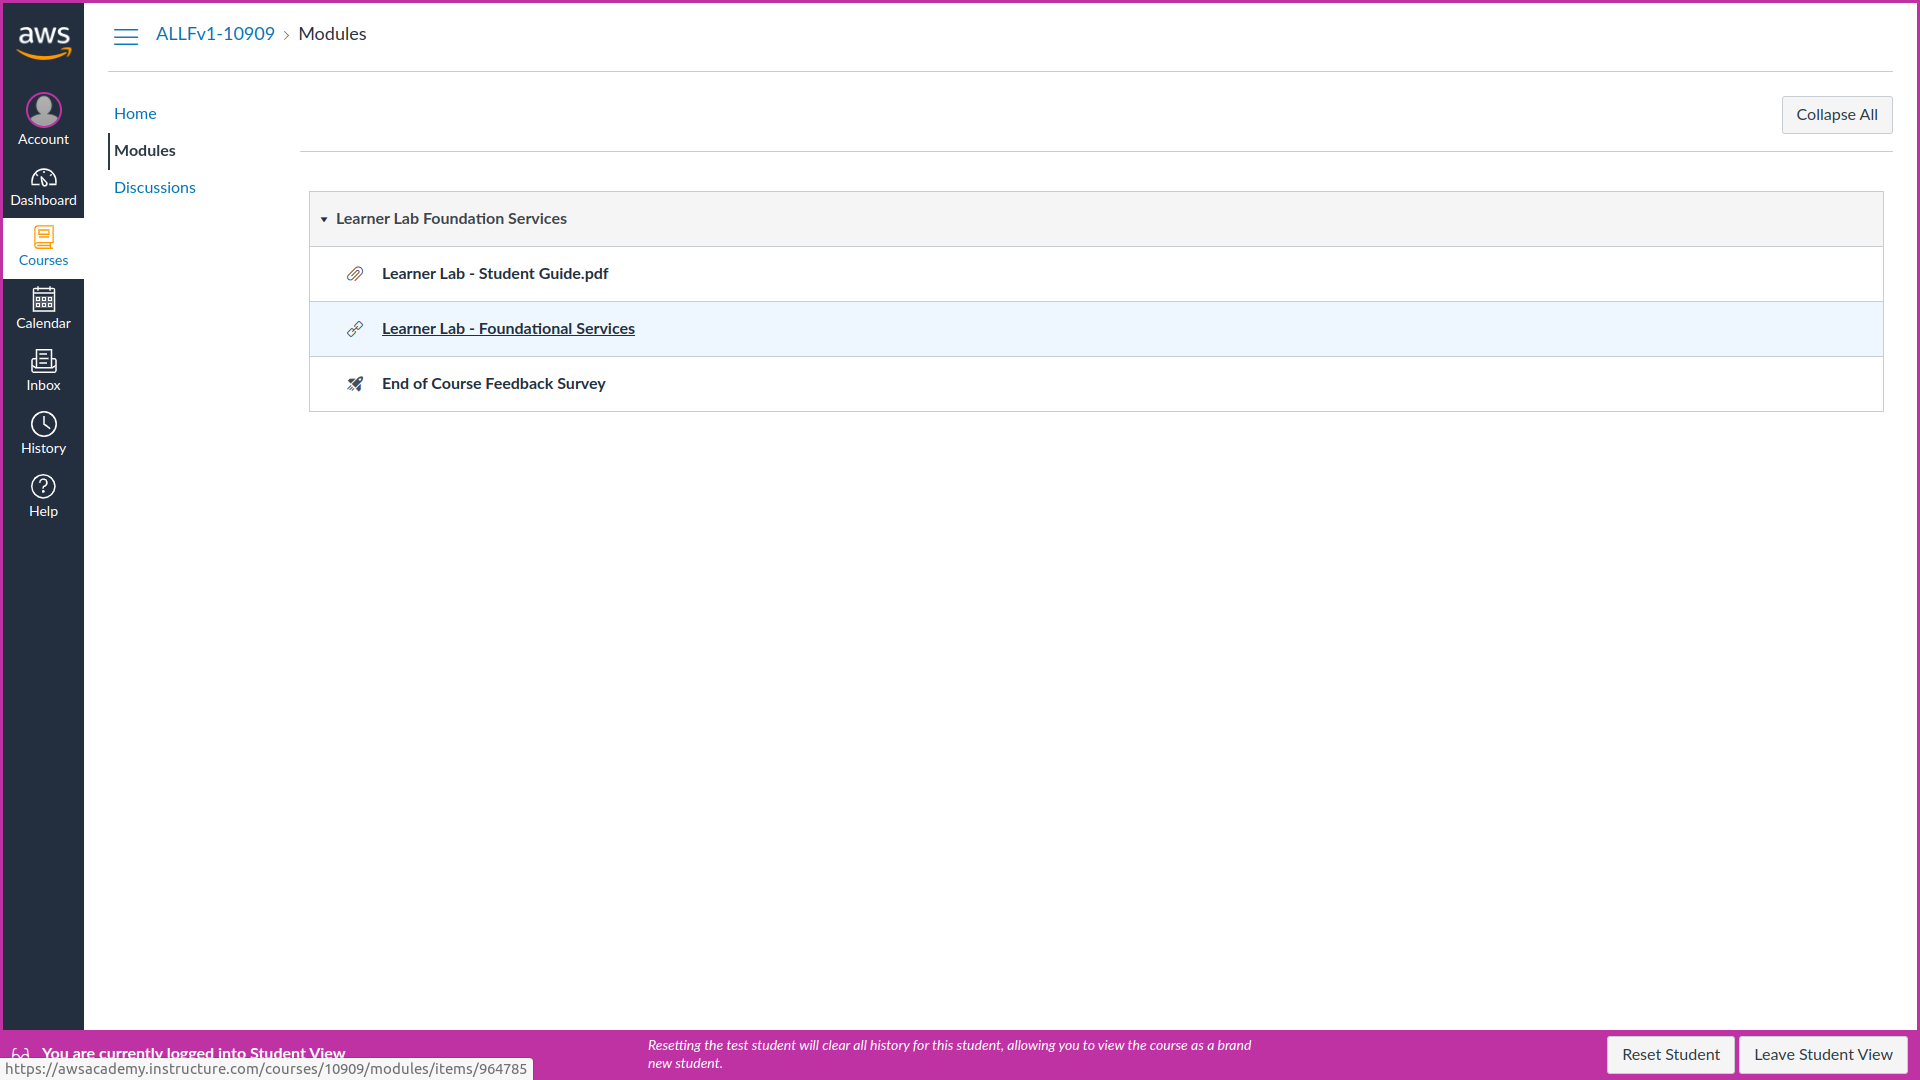
\includegraphics[width=0.9\textwidth]{images/modules-page}

\item Now we have entered the main part of the interface, the learner lab.
\begin{itemize}
      \item The AWS text with the currently red circle is the link to open the AWS console.
      \item You also see your budget, note that the budget is not updated in real-time.
      \item The \texttt{00:00} indicates how long your lab has been activated.
      A lab can only remain active for 6 hours, after which it will be closed, unless you press start lab again before the 6 hours expires.
      \item AWS details will become important later but are not needed now.
      \item The README button will re-open the text panel currently on the right of the terminal interface.
      \item The terminal interface is not important.
      \item The right-hand has a lot of important information including what AWS services are available in the learner labs environment, please read it.
\end{itemize}

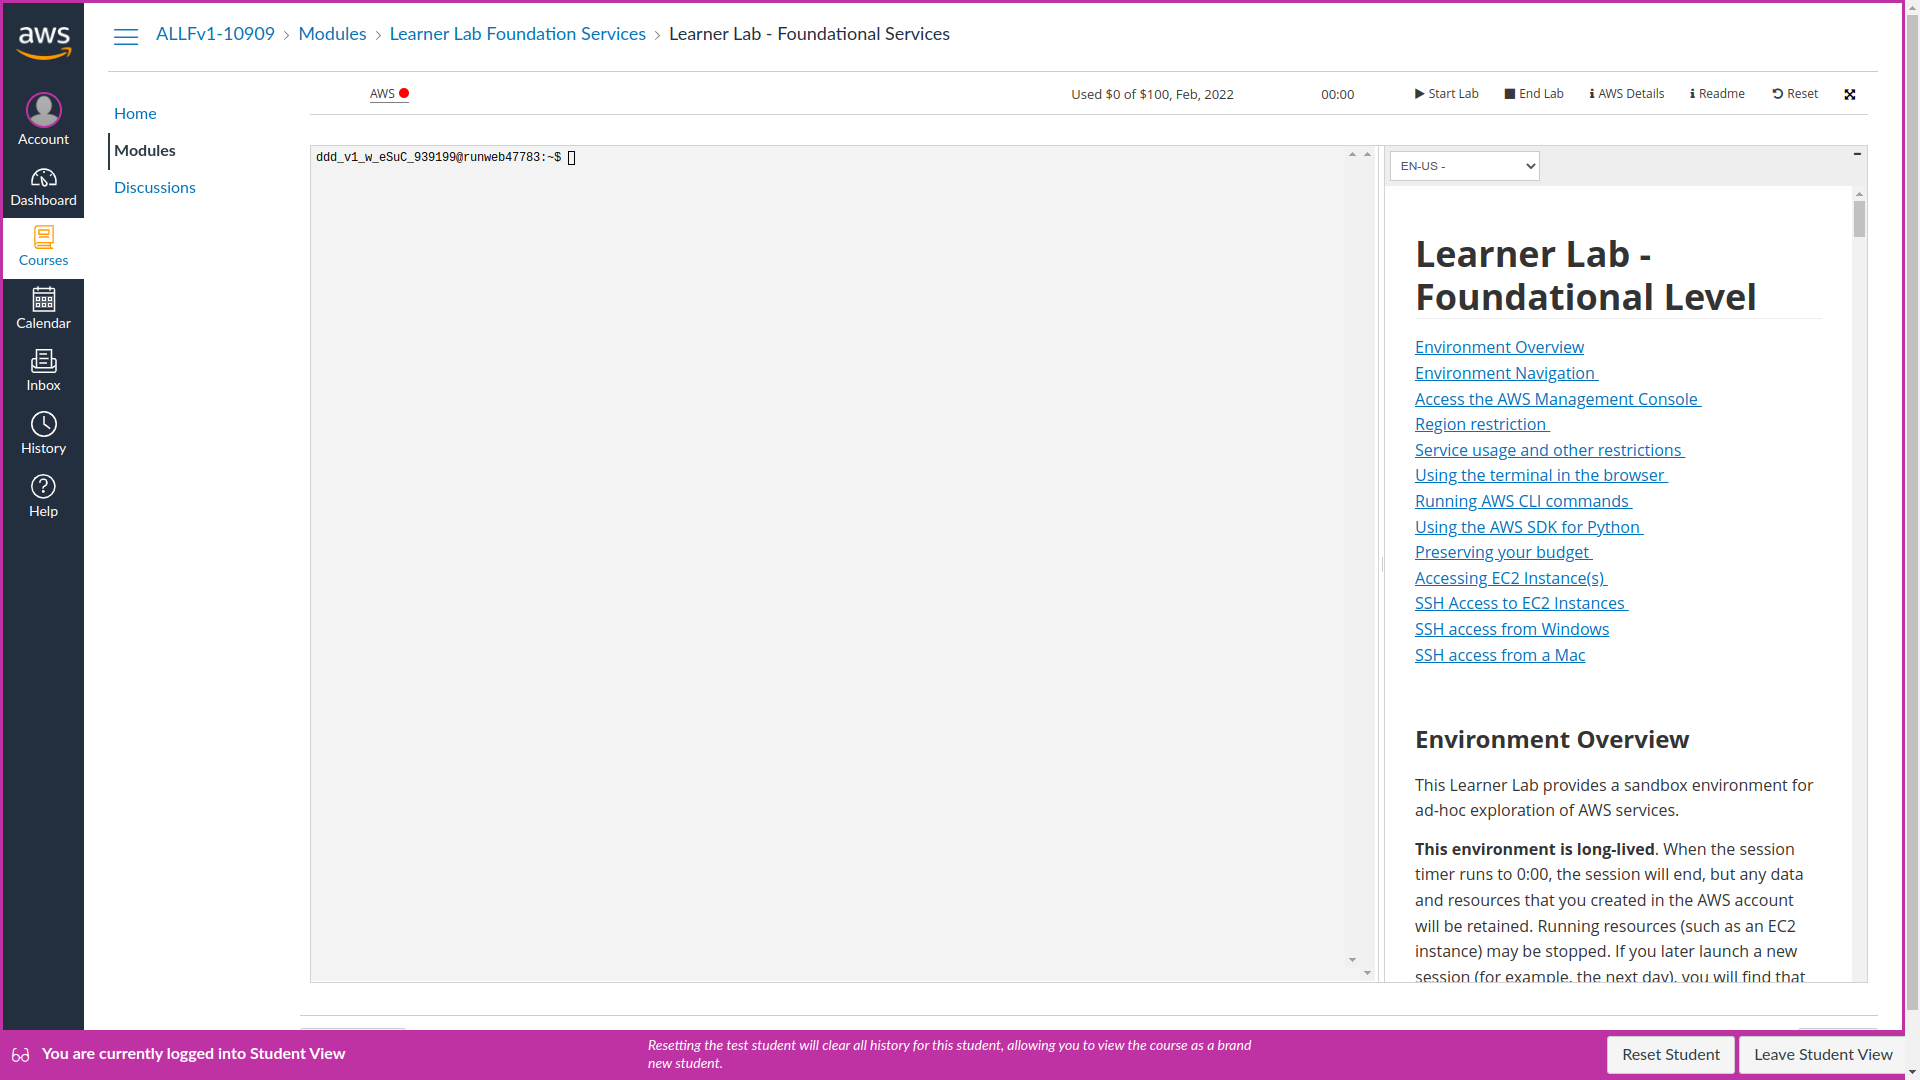
\includegraphics[width=0.9\textwidth]{images/lab-interface}

\item Go ahead and start the lab. It will take a few moments to get ready and the red circle will turn green once it is.
      Click on the green circle when it is available.
      This will open the AWS Console in a new tab.\footnote{Your view will be different as you will not yet have any recently visited services.}
      If you end up working in a company which uses AWS, welcome to your new home.

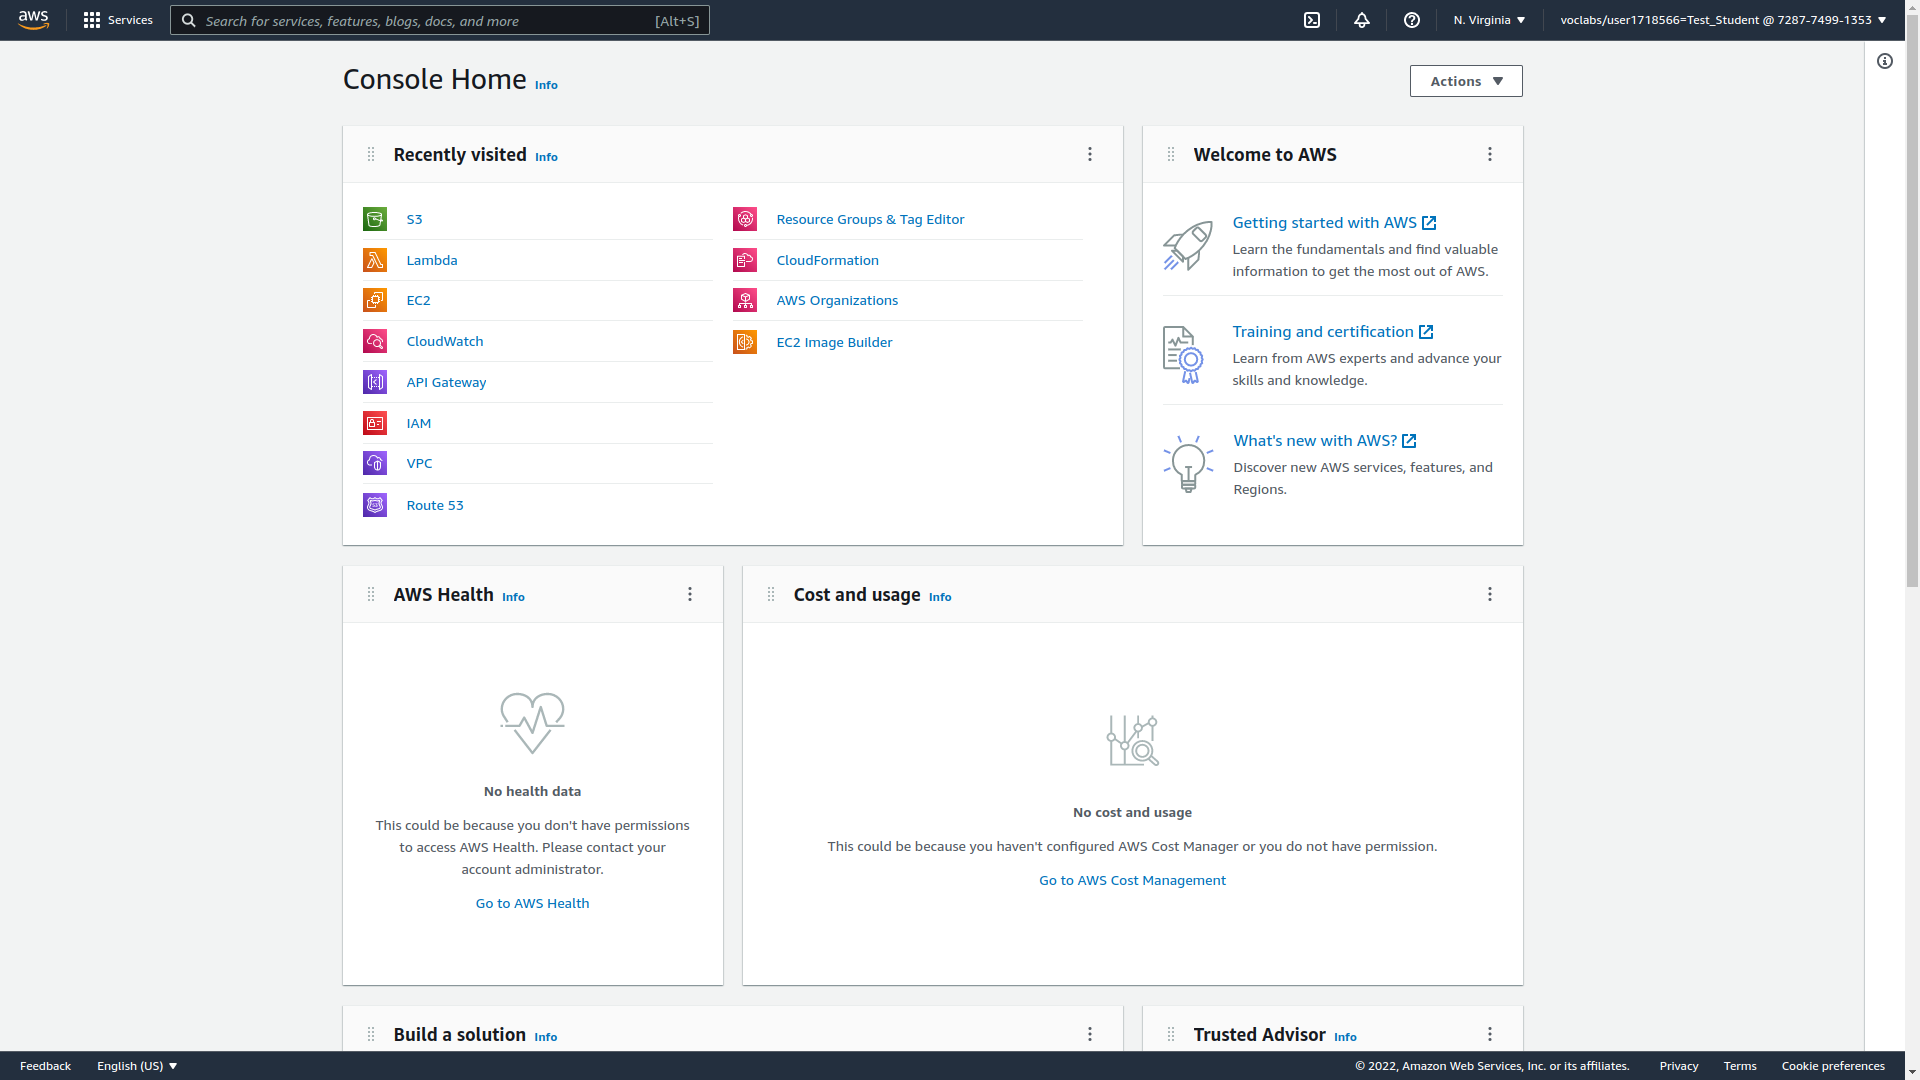
\includegraphics[width=0.9\textwidth]{images/aws-console}

\end{enumerate}

\aside{A short introduction to AWS:
Amazon Web Services (AWS) is an Infrastructure as a Service (IaaS) provider.
They offer a collection of services which are helpful for development.
For example, they offer virtual compute resources, database storage options, and networking to tie it all together.
Services are offered with a pay as you go model, meaning you only pay for the seconds you use a service.
We will get acquainted with some simple services offered by AWS now.}

\section{AWS EC2}

Today we are going to focus on using AWS's EC2 service.
Elastic Compute Cloud (EC2) is the primary compute service offered by AWS.
It allows you to create a linux virtual machine on Amazon's infrastructure.
You have full control over this machine and can configure it for whatever purpose you need.

Navigate to the search bar in the top left and find the EC2 service.
You might find this interface overwhelming.
It is important to note that since EC2 is one of the primary services offered by AWS,
many smaller services we do not need are bundled into the service.

\vspace{3mm}
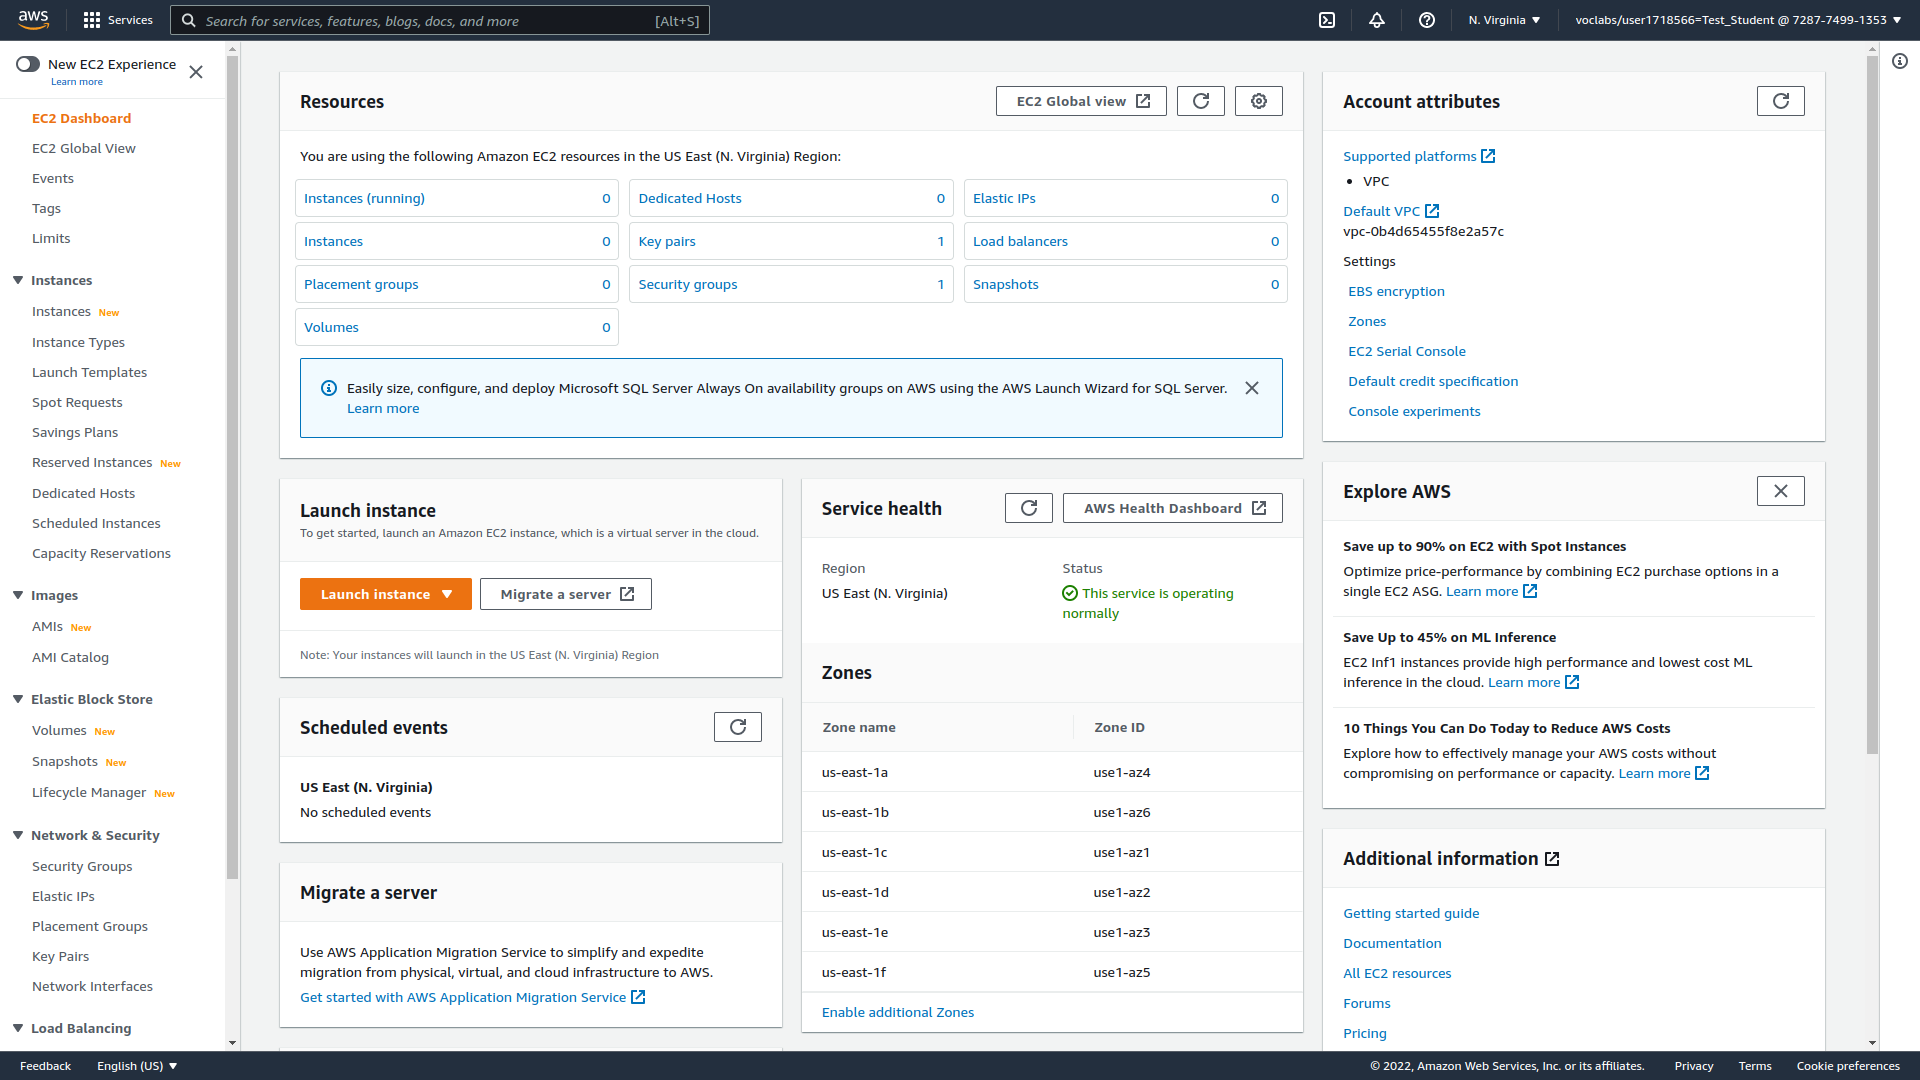
\includegraphics[width=0.9\textwidth]{images/ec2-interface}
\vspace{3mm}

Today, we will just need the \texttt{Instances} dashboard.
Navigate to there and select ``Launch instances''.

\subsection{EC2 AMI}
First we will need to select an Amazon Machine Image (AMI).
An AMI is the template (cookie cutter) which provides instructions on how an instance should be provisioned.
Amazon offers a range of built-in AMIs. There are also community AMIs or you can create your own.
As we just want a simple server today, we will use one of the built-in AMIs.

Every AMI has a unique AMI code, something that looks like \texttt{ami-0a8b4cd432b1c3063}.
We will use this AMI today%
\footnote{Check the requirements for your chosen website, if your website requires a specific operating system, look for it as a community AMI.
Ask for help if you aren't sure.}
, it is considered one of the fundamental images.
Search for it via the code and select it.

\subsection{Instance Settings}
The next few settings for configuring your instance are:
\begin{enumerate}
\item We do not need a large server, choose \texttt{t2.micro}.
\item Keep the `Configure Instance' settings as default.
\item Keep the `Add Storage' settings as default.
\item Add a `Name' tag, call it the name of your website, e.g. \texttt{hextris}.
\item Choose `Create a \textbf{new} security group'.
\begin{enumerate}
\item Give it a meaningful name, e.g. \texttt{hextris-http-ssh-access}.
\item Change the description to something meaningful, e.g. \texttt{Hextris HTTP and SSH access}.
\item Add a rule, select the \texttt{Type} as \texttt{HTTP}.
\end{enumerate}
\item When asked to choose a key pair, select the existing \texttt{vockey | RSA} option.
\end{enumerate}

\section{Accessing the Instance}

Return to the \texttt{Instances} dashboard.
You should now see a new instance created, its instance state might not yet be \texttt{Running}, if not, wait.

\vspace{1mm}
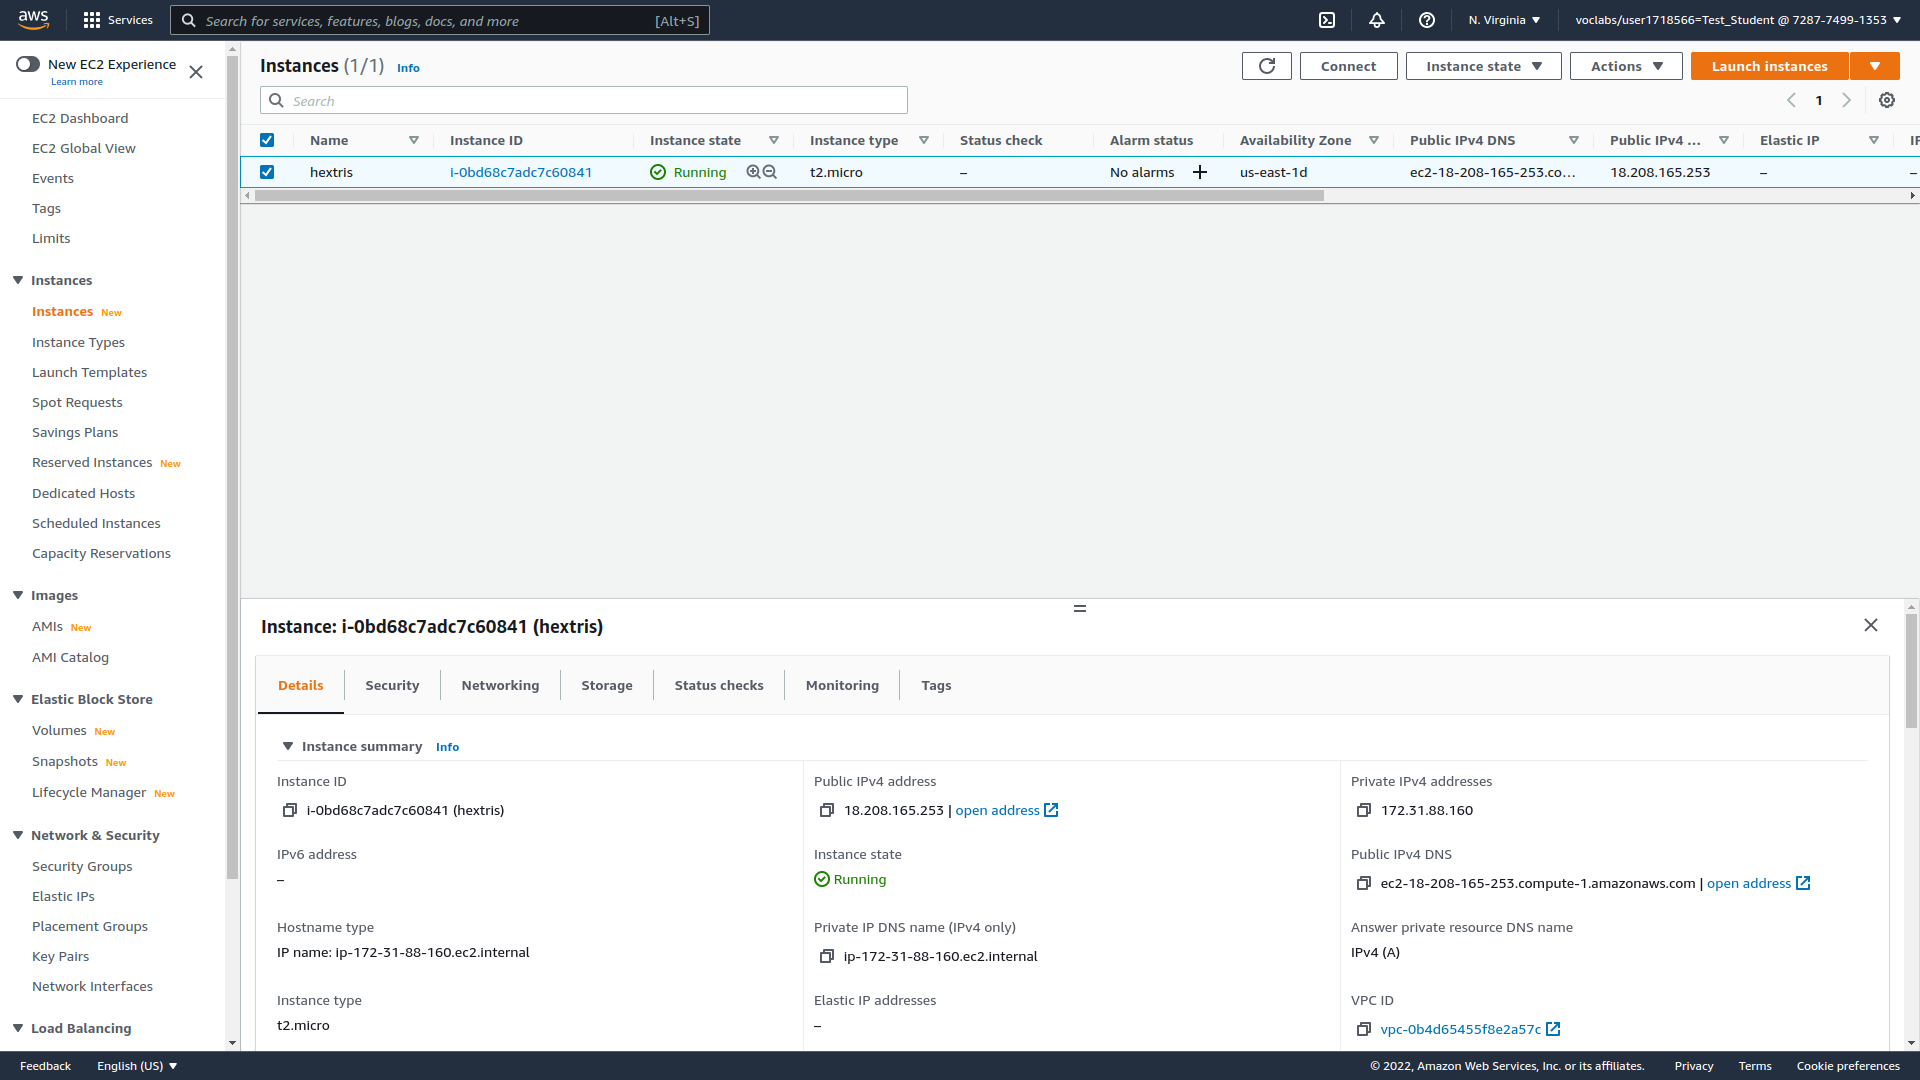
\includegraphics[width=0.9\textwidth]{images/instance-interface}

Note the public IPv4 address, we will need to use this to connect to the server.

\begin{enumerate}
    \item Return to the learner lab interface.
    \item Run the following, replacing \texttt{127.0.0.1} with the public IP of your instance.
          This command uses the \texttt{vockey | RSA} key pair to gain SSH access to the machine.
\end{enumerate}
\bash{ssh -i ~/.ssh/labsuser.pem ec2-user@127.0.0.1}

\section{Installing Hextris}
Hextris is very simple to install, using an EC2 interface is perhaps overkill for it.
It is an entirely client-side application which means we just have to serve the static files.

First, we will need to enable the basic serving of static files.
We can install and start the \texttt{httpd} service for this.
The AMI we have picked uses the yum package manager, so to install httpd we run:

\bash{sudo yum install httpd^^J
\$ sudo systemctl enable httpd^^J
\$ sudo systemctl start httpd
}

All files in the \texttt{/var/www/html} directory will now be served when accessed via HTTP.
Change to this directory and notice that it is currently empty.

Next, we need to download the static files to the server.
We can use git for this, but first git needs to be installed on the machine.

\bash{sudo yum install git}

Finally, let's double check we are in the \texttt{/var/www/html} directory.

\bash{cd /var/www/html}

And clone the repository into that directory.

\bash{sudo git clone https://github.com/Hextris/hextris .}

Now if you navigate to the \textbf{http} address of the public IP address (e.g. \url{http://18.208.165.253}), you should be able to see your newly deployed website.

\section{Further Work}
If you picked your own website to deploy, the steps for installation will likely be more involved.
Track down those instructions and try your best to deploy the site.
If you get stuck, ask your neighbour or your tutor.

Once you have worked out how to deploy your chosen website,
please commit an installation script or installation instructions for others to re-use:
\url{https://github.com/CSSE6400/selfhost-cookbook}

\bibliographystyle{ieeetr}
\bibliography{hextris}

\end{document}